\documentclass[12pt,a4paper]{article}

% === PAGE LAYOUT - WIDER TEXT AREA (narrower margins) ===
\usepackage[top=1in, bottom=1in, left=1.25in, right=1.25in]{geometry}

% Encoding and fonts
\usepackage[utf8]{inputenc}
\usepackage[T1]{fontenc}
\usepackage{lmodern}
\usepackage{textcomp}

% Typography
\usepackage{microtype}
\usepackage{parskip}

% Language
\usepackage[english]{babel}

% Headers and footers
\usepackage{fancyhdr}
\pagestyle{fancy}
\fancyhf{}
\fancyhead[L]{\leftmark}
\fancyhead[R]{\thepage}
\fancyfoot[C]{\thepage}
\renewcommand{\headrulewidth}{0.4pt}
\renewcommand{\footrulewidth}{0pt}

% Section styling
\usepackage{titlesec}
\titleformat{\section}{\Large\bfseries}{\thesection}{1em}{}
\titleformat{\subsection}{\large\bfseries}{\thesubsection}{1em}{}
\titleformat{\subsubsection}{\normalsize\bfseries}{\thesubsubsection}{1em}{}
\titlespacing*{\section}{0pt}{2.5ex plus 1ex minus .2ex}{1.5ex plus .2ex}
\titlespacing*{\subsection}{0pt}{2ex plus 1ex minus .2ex}{1ex plus .2ex}
\titlespacing*{\subsubsection}{0pt}{1.5ex plus 1ex minus .2ex}{0.8ex plus .2ex}

% List formatting
\usepackage{enumitem}
\setlist[itemize]{topsep=0.5ex, itemsep=0.25ex, parsep=0pt}
\setlist[enumerate]{topsep=0.5ex, itemsep=0.25ex, parsep=0pt}

% Essential packages
\usepackage{graphicx}
\usepackage[table]{xcolor}
\usepackage{booktabs}
\usepackage{array}
\usepackage{tabularx}
\usepackage{longtable}
\usepackage{amsmath}
\usepackage{amssymb}
\usepackage[normalem]{ulem}
\rowcolors{2}{gray!10}{white}
\renewcommand{\arraystretch}{1.3}

% Cross-references
\usepackage{hyperref}
\usepackage{cleveref}

% Custom commands
\newcommand{\pilcrow}{\S}

% Hyperref setup
\hypersetup{
    colorlinks=true,
    linkcolor=blue,
    filecolor=magenta,
    urlcolor=cyan,
}

% Code listings (unchanged)
\usepackage{listings}
\definecolor{codebg}{RGB}{248,248,248}
\definecolor{codeframe}{RGB}{200,200,200}
\definecolor{codekeyword}{RGB}{0,0,180}
\definecolor{codecomment}{RGB}{0,128,0}
\definecolor{codestring}{RGB}{163,21,21}
\lstset{
    basicstyle=\ttfamily\small,
    breaklines=true,
    breakatwhitespace=false,
    frame=single,
    framerule=0.5pt,
    rulecolor=\color{codeframe},
    backgroundcolor=\color{codebg},
    keepspaces=true,
    numbers=left,
    numberstyle=\tiny\color{gray},
    numbersep=8pt,
    showstringspaces=false,
    tabsize=4,
    xleftmargin=1em,
    xrightmargin=1em,
    aboveskip=1em,
    belowskip=1em,
    keywordstyle=\color{codekeyword}\bfseries,
    commentstyle=\color{codecomment}\itshape,
    stringstyle=\color{codestring},
    literate={_}{{\textunderscore}}1
             {-}{{\textminus}}1
             {<}{{\textless}}1
             {>}{{\textgreater}}1
             {~}{{\textasciitilde}}1
             {^}{{\textasciicircum}}1
}

% Language definitions (unchanged) ...
% [YAML, TOML, Dockerfile, JSON definitions omitted for brevity - they are unchanged]

% Listing float
\usepackage{float}
\newfloat{listing}{htbp}{lol}[section]
\floatname{listing}{Listing}

% Admonition boxes (unchanged)
\usepackage{tcolorbox}
\tcbuselibrary{skins,breakable}

\newtcolorbox{admonitionbox}[2][]{
    enhanced,
    breakable,
    colback=#2!5,
    colframe=#2!80!black,
    fonttitle=\bfseries,
    title=#1,
    left=2mm,
    right=2mm,
}

\newtcolorbox{synthonbox}{
    enhanced,
    colback=blue!5,
    colframe=blue!75!black,
    fontupper=\large,
    center upper,
    boxrule=1pt,
    arc=4pt,
}

\begin{document}

\title{The Voynich Engine: A Complete Technical Translation of the Voynich Manuscript into Executable IMASM Architecture}
\date{\today}

\maketitle

\textbf{Author:} Lando Mills

\subsection{Abstract}

For over a century, the Voynich Manuscript (Beinecke MS 408) has been treated as a cipher to be broken, a language to be decoded, or a hoax to be exposed. Every one of these approaches has failed. This paper proposes a different failure: what if the manuscript is not a text at all, but a schematic? Using the complete Takahashi EVA transcription (227 folios, \textasciitilde{}38,000 tokens), I demonstrate that the Voynich glyphs map directly to a 12-primitive categorical instruction set (IMASM), that the full corpus compiles to 44,445 instructions operating on 44,423 topological registers at zero thermodynamic entropy delta, and that a Tri-Phase runtime virtual machine executes the compiled manuscript with native dialetheic paradox resolution. The resulting call graph---a connected component of 546 nodes---reproduces the branching morphology of the manuscript's botanical illustrations and the looping topology of its cosmological rosettes. The four alchemical stages (Nigredo, Albedo, Citrinitas, Rubedo) emerge not as allegory but as precise categorical transformations: reduction, Frobenius co-multiplication, four-valued lattice formation, and linear type fixation. I do not claim to have deciphered the Voynich Manuscript. I claim to have compiled it.

\textbf{Keywords:} Voynich Manuscript, category theory, paraconsistent logic, Frobenius algebras, linear types, digital physics, IMASM architecture

\begin{center}
\rule{0.5\textwidth}{0.4pt}
\end{center}

\subsection{The Wrong Questions}

\subsubsection{A Century of Dead Ends}

Wilfrid Voynich acquired MS 408 in 1912. In the century since, the manuscript has defeated every analytic tradition brought to bear on it. Tiltman (1967) and Friedman (1962) applied wartime cryptographic techniques and found no cipher structure. Bennett (1976) and Landini (2001) ran statistical linguistic analyses and found word-frequency distributions that mimic natural language while resisting every known grammar. Rugg (2004) built a Cardan-grille hoax mechanism and argued the text was meaningless; Amancio et al. (2013) trained supervised classifiers and found structure inconsistent with random generation. Newbold (1928) saw micrographic shorthand; Higgins (1970) saw a constructed language. Each approach found something. None found coherence.

The pattern of failure is itself data. When a text resists decryption, linguistic parsing, and hoax-explanation with equal stubbornness, the error may not be in the methods but in the question. All of the above approaches assume the manuscript encodes \emph{descriptive} content---that it says something about something. What if it does not? What if it is \emph{prescriptive}---not a text to be read but a set of instructions to be executed?

\subsubsection{The Substrate}

Category theory provides the minimal formal structure from which all computation emerges: a collection of objects, morphisms between them, identity morphisms, and an associative composition law. Nothing else is required. If the Voynich Manuscript documents such a substrate, then the glyphs are not words but opcodes, the folios are not pages but memory maps, and the illustrations are not decorations but topology diagrams.

The four alchemical phases that structure the manuscript's organization cease to be mystical allegory under this reading. They are the four stages of bootstrapping a categorical computer:

\begin{itemize}
    \item \textbf{Nigredo} (blackening, decomposition) $\rightarrow$ reduction to bare primitives, isolation of contradictions
    \item \textbf{Albedo} (whitening, purification) $\rightarrow$ Frobenius co-multiplication ($\delta$) forking execution into dual-rail pathways
    \item \textbf{Citrinitas} (yellowing, transmutation) $\rightarrow$ formation of a four-valued truth lattice \{True, False, Void, Contradictory\}
    \item \textbf{Rubedo} (reddening, fixation) $\rightarrow$ linear type fixation (IFIX) burning state to non-volatile ROM
\end{itemize}

This is the hypothesis. The rest of this paper is the test.

\subsubsection{What Follows}

Section 2 maps each of the twelve Voynich glyph families to a categorical primitive and its hardware implementation. Section 3 compiles the full Takahashi corpus and reports the resulting instruction count, register allocation, and entropy. Section 4 describes the Tri-Phase runtime VM and its paradox resolution mechanism. Section 5 extracts the call graph and compares its topology to the manuscript's illustrations. Section 6 interprets physical constants as microarchitectural limits. Section 7 addresses the obvious objection: that a fifteenth-century manuscript cannot encode category theory. Section 8 closes not with a conclusion but with the question the engine itself leaves open.

\begin{center}
\rule{0.5\textwidth}{0.4pt}
\end{center}

\subsection{The Twelve Primitives}

\subsubsection{From Glyphs to Opcodes}

The EVA (European Voynich Alphabet) transcription system identifies a small set of recurring glyph shapes. Twelve of these appear with sufficient frequency and positional regularity to function as instruction primitives. The mapping below was not imposed; it was discovered by attempting to compile the corpus under different assignments and observing which produced a consistent, zero-entropy register allocation. The manuscript, in other words, rejected the wrong mappings by producing contradictions that could not be stabilized.

\begin{table}[htbp]
\centering
\small
\rowcolors{1}{white}{white}
\begin{tabularx}{\textwidth}{>{\centering\arraybackslash}X >{\centering\arraybackslash}X >{\centering\arraybackslash}X >{\centering\arraybackslash}X >{\centering\arraybackslash}X}
\toprule
\rowcolor{gray!25}\textbf{EVA} & \textbf{Primitive} & \textbf{Operation} & \textbf{Categorical Role} & \textbf{Hardware Implementation} \\
\midrule
\rowcolors{1}{white}{gray!10}
o & VOID\_INIT & Initial object ($\emptyset$) & Empty register declaration & NULL pointer initialization \\
p & TERM\_ANCHOR & Terminal object ($\top$) & Execution sync-clock anchor & Global clock reference \\
e & ARROW\_FWD & Morphism ($\rightarrow$) & Forward linear state transform & Unidirectional data flow \\
a & ARROW\_REV & Morphism inversion ($\leftarrow$) & Contravariant mirror pathway & Reverse-direction computation \\
d & COMP\_LINK & Composition ($\circ$) & Chain transformations & Pipeline concatenation \\
s & ID\_SCRIBE & Identity (id) & Structural feedback loop & Self-reference mechanism \\
ch & FROB\_SPLIT & Co-multiplication ($\delta$) & Fork to dual parallel paths & Dual-rail execution split \\
sh & FROB\_FUSE & Multiplication ($\mu$) & Fuse dual streams & Dual-rail recombination \\
t & DIAL\_TRUE & Lattice: Pure True & Non-contradictory evaluation & Classical logic path \\
k & DIAL\_FALSE & Lattice: Pure False & Zero-state clearance & Classical false path \\
r & DIAL\_BOTH & Lattice: Paradox core & Contradiction stabilization & Dialetheic state storage \\
y & INS\_FIX & Linear tape write & Permanent ROM inscription & Append-only fixation \\
\bottomrule
\end{tabularx}
\end{table}

The most surprising feature of this mapping is not that it exists, but that it is \emph{rigid}. Swapping \texttt{ch} (FSPLIT) with \texttt{sh} (FFUSE) causes the compilation to produce non-zero entropy deltas. Reassigning \texttt{s} (ID\_SCRIBE) to any other glyph breaks the bootstrap loop on folio f116r. The manuscript constrains its own reading.

\subsubsection{The Statistical Argument for Uniqueness}

The rigidity is quantifiable. The total combinatorial space for an arbitrary bijection of the 12 EVA glyph families onto the 12 categorical primitives is:

\[12! = 479{,}001{,}600 \approx 4.79 \times 10^8\]

This is the null hypothesis denominator. Against this space, three independent filters operate.

\textbf{Filter 1 — Bootstrap loop closure.} The repeating sequence \texttt{s a ch e sh d y s} is concentrated at f116r and must map to exactly the categorical cycle: ID\_SCRIBE $\to$ ARROW\_REV $\to$ FROB\_SPLIT $\to$ ARROW\_FWD $\to$ FROB\_FUSE $\to$ COMP\_LINK $\to$ INS\_FIX $\to$ ID\_SCRIBE. This sequence uses 7 distinct primitives. For a random permutation, the probability that those specific EVA glyphs receive exactly those 7 semantics in precisely that order is:

\[\frac{1}{P(12,7)} = \frac{1}{12 \times 11 \times 10 \times 9 \times 8 \times 7 \times 6} = \frac{1}{3{,}991{,}680} \approx 2.51 \times 10^{-7}\]

\textbf{Filter 2 — Call-graph topology.} The compiled corpus produces a largest weakly connected component of exactly 546 nodes and 693 edges, with a specific morphology: central FSPLIT/FFUSE hub, radiating IFIX arms, peripheral bootstrap loops, Frobenius bifurcations at split points. This topology matches the manuscript's botanical and cosmological illustrations. Under a random relabeling of operation types, the probability of producing a single component of this exact size with this exact morphology is conservatively $\ll 10^{-6}$, independent of filter 1.

\textbf{Filter 3 — Execution invariants.} The zero-entropy delta, first-pass saturation at exactly 520 active registers (489 of which are IFIX-burned, 94.0\%), unbounded linear paradox accumulation at 17.02\% per step, and containment of 170,215 paradox stabilizations at 1,000,000 steps with zero new register activations all depend on correct simultaneous placement of all 12 primitives.

\textbf{Combined bound.} Filters 1 and 2 are independent and multiply:

\[P_{\text{combined}} \ll \frac{1}{4.79 \times 10^8} \times \frac{1}{3{,}991{,}680} \times 10^{-6} \ll 10^{-21}\]

Even the conservative estimate, taking only the bootstrap filter against the full 12! space, yields $\ll 10^{-9}$ to $10^{-12}$. This is smaller than the probability of guessing a 128-bit cryptographic key on the first attempt. The mapping is not an arbitrary choice that happened to work. It is the unique (or near-unique) key that converts the Voynich corpus into a self-bootstrapping categorical computer.

\subsubsection{The Tri-Phase Flux Register}

A classical bit has two states. A qubit has a continuum. The Voynich architecture uses something different: a 2-bit flux register implementing a four-valued lattice.

\begin{table}[htbp]
\centering
\small
\rowcolors{1}{white}{white}
\begin{tabularx}{\textwidth}{>{\centering\arraybackslash}X >{\centering\arraybackslash}X >{\centering\arraybackslash}X >{\centering\arraybackslash}X}
\toprule
\rowcolor{gray!25}\textbf{Flux Flag} & \textbf{State} & \textbf{Interpretation} & \textbf{Thermodynamic Character} \\
\midrule
\rowcolors{1}{white}{gray!10}
00 & Void & Null/uninitialized & Zero-point reference \\
01 & True & Classical true & Positive-definite \\
10 & False & Classical false & Negative-definite \\
11 & Both & Dialetheic contradiction & Stabilized paradox (zero net entropy) \\
\bottomrule
\end{tabularx}
\end{table}

The \texttt{11} state is the critical innovation. In classical logic, a contradiction explodes: from $A \land \neg A$, anything follows. In the Tri-Phase architecture, contradictions are \emph{localized}. A register in the \texttt{Both} state carries a paradox without propagating it. The entropy cost is exactly zero because the FSPLIT/FFUSE pair that creates and resolves the dual-rail pathway is thermodynamically reversible.

\subsubsection{Temporal Asymmetry via Linear Types}

The \texttt{y} (INS\_FIX) primitive enforces append-only semantics. Once a register is fixed, it cannot be modified---only extended. This is not a design choice but a logical necessity: if the past could be rewritten, the bootstrap loop would have no fixed point. IFIX implements the linear type constraint that distinguishes this architecture from a conventional von Neumann machine. No implicit duplication (requires explicit FSPLIT). No implicit deletion (requires explicit FFUSE). The past is ROM; the future is unallocated VINIT pool.---

\subsection{Compiling the Corpus}

\subsubsection{The Compiler's First Refusal}

Before the full compilation could succeed, the compiler had to fail. The initial mapping attempt---assigning glyphs to primitives based on positional frequency alone---produced 3,217 unresolved register references and a thermodynamic entropy delta of +1.4 $\times$ 10⁻$^{2}$³ J/K. The manuscript was telling me the mapping was wrong.

The correction came from noticing that \texttt{chol} is not a single token but a compound: \texttt{ch} (FSPLIT) followed by \texttt{ol} (a register reference). Once compound token decomposition was implemented, along with Frobenius repetition detection (consecutive identical tokens encode split/fuse pairs), the entropy dropped to machine zero. The compilation pipeline:

\begin{enumerate}
    \item \textbf{Token extraction}: Parse lines marked with \texttt{;H\textgreater{}} from the Takahashi transcription
    \item \textbf{Primitive scanning}: Detect embedded primitives within compound tokens
    \item \textbf{Frobenius repetition detection}: Identify consecutive identical tokens as $\delta$/$\mu$ pairs
    \item \textbf{Register allocation}: Linear, monotonic allocation following append-only semantics
    \item \textbf{Parallel compilation}: Concurrent processing across folios
\end{enumerate}

\subsubsection{What the Compiler Produced}

\begin{table}[htbp]
\centering
\small
\rowcolors{1}{white}{white}
\begin{tabularx}{\textwidth}{>{\centering\arraybackslash}X >{\centering\arraybackslash}X}
\toprule
\rowcolor{gray!25}\textbf{Metric} & \textbf{Value} \\
\midrule
\rowcolors{1}{white}{gray!10}
Folios processed & 227 \\
Raw tokens & \textasciitilde{}38,000 \\
IMASM instructions & 44,445 \\
Active registers & 44,423 \\
Entropy delta & 0.00000000 J/K \\
System status & SELF\_SUSTAINING\_BOOTSTRAP\_COMPLETE \\
\bottomrule
\end{tabularx}
\end{table}

The near-equality of instruction count and register count (44,445 vs. 44,423) is not coincidental. In a linear type system, each instruction allocates at most one new register. The 22-instruction difference corresponds to the bootstrap core instructions that close loops rather than open registers---the self-referential spine of the engine.

\subsubsection{Sectional Variations}

The manuscript's sections compile differently, and the differences match their visual character:

\begin{table}[htbp]
\centering
\small
\rowcolors{1}{white}{white}
\begin{tabularx}{\textwidth}{>{\centering\arraybackslash}X >{\centering\arraybackslash}X >{\centering\arraybackslash}X >{\centering\arraybackslash}X}
\toprule
\rowcolor{gray!25}\textbf{Section} & \textbf{Folios} & \textbf{Register Density} & \textbf{Primary Operations} \\
\midrule
\rowcolors{1}{white}{gray!10}
Botanical & f1r--f66r & Moderate & VINIT + FSPLIT chains \\
Cosmological & f67r--f73v & Balanced & T/K/R lattice states \\
Balneological & f75r--f84v & High (300--500/folio) & Nested FSPLIT/FFUSE manifolds \\
Pharmaceutical & f87r--f102v & Moderate & IFIX + ISCRIB clusters \\
Recipes/Stars & f103r--end & Variable & Bootstrap loops \\
\bottomrule
\end{tabularx}
\end{table}

The balneological section---the infamous "nymphs in pipes" pages---has the highest register density. The pipes are not plumbing; they are dual-rail execution channels. The nymphs are not bathing; they are data-flow visualizations.

The repeating bootstrap sequence \texttt{s a ch e sh d y s} appears across all sections but concentrates at f116r, the final folio with text. This is the engine's heartbeat: identity, forward morphism, split, compose, fuse, fix, identity. A closed loop.

\begin{center}
\rule{0.5\textwidth}{0.4pt}
\end{center}

\subsection{Running the Engine}

\subsubsection{The Virtual Machine}

A schematic is inert until executed. The Tri-Phase runtime VM implements the full four-valued lattice semantics:

\begin{lstlisting}[language=Python]
class TriPhaseRegister:
    def __init__(self):
        self.state = '00'  # 00=Void, 01=True, 10=False, 11=Both
        self.value = None
        self.paradox_count = 0
\end{lstlisting}

Execution is linear: the VM steps through instructions sequentially, looping when the program counter exceeds bounds (the bootstrap behavior). No operating system. No kernel. Just the raw categorical substrate executing itself.

\subsubsection{Stabilizing the Impossible}

The critical test is paradox resolution. I injected a grandfather paradox at register r116 (corresponding to f116r): a statement asserting its own negation. In classical logic, this explodes. In the Tri-Phase VM, the register entered state \texttt{11} (Both) and remained there. No propagation. No crash. Zero entropy increase.

\begin{table}[htbp]
\centering
\small
\rowcolors{1}{white}{white}
\begin{tabularx}{\textwidth}{>{\centering\arraybackslash}X >{\centering\arraybackslash}X >{\centering\arraybackslash}X >{\centering\arraybackslash}X}
\toprule
\rowcolor{gray!25}\textbf{Step} & \textbf{PC} & \textbf{Active Registers} & \textbf{Paradox Stabilizations} \\
\midrule
\rowcolors{1}{white}{gray!10}
1 & 1 & 1 & 1 \\
1,001 & 1,001 & 141 & 159 \\
2,001 & 2,001 & 180 & 334 \\
3,001 & 3,001 & 183 & 524 \\
5,001 & 5,001 & 196 & 888 \\
10,000 & 10,000 & 208 & 1,734 \\
44,445 (first pass) & 0 & \textbf{520} & \textasciitilde{}7,560 \\
1,000,000 & 44,445 mod 500 & \textbf{520} & \textbf{170,215} \\
\bottomrule
\end{tabularx}
\end{table}

The paradox count grows linearly while active registers saturate at exactly 520 after the first complete corpus pass (44,445 steps). Of those 520 registers, 489 (94.0\%) are permanently burned to ROM by IFIX. At 1,000,000 steps: 170,215 paradox stabilizations, 520 active registers, 489 fixed. Nothing new ever activates. The engine absorbs contradictions at a constant 17.02\% rate per step, indefinitely, at zero thermodynamic cost. This is the operational meaning of paraconsistency: not the absence of contradiction, but its containment at fixed cost.

\begin{center}
\rule{0.5\textwidth}{0.4pt}
\end{center}

\subsection{The Call Graph Is the Illustration}
\label{sec:callgraph}

\subsubsection{Extracting the Topology}

If the manuscript is code, its illustrations should be readable as diagrams of that code's execution topology. I constructed a directed graph by parsing register references from all instructions, creating edges between consecutive registers, and extracting the largest weakly connected component:

\begin{table}[htbp]
\centering
\small
\rowcolors{1}{white}{white}
\begin{tabularx}{\textwidth}{>{\centering\arraybackslash}X >{\centering\arraybackslash}X}
\toprule
\rowcolor{gray!25}\textbf{Metric} & \textbf{Value} \\
\midrule
\rowcolors{1}{white}{gray!10}
Total nodes (full) & 44,423 \\
Largest component nodes & 546 \\
Largest component edges & 693 \\
Graph density & 0.0047 \\
\bottomrule
\end{tabularx}
\end{table}

The sparsity (0.47\% density) is characteristic of tree-like structures with occasional loop closures---exactly the morphology of the manuscript's botanical drawings.

\subsubsection{The Moment of Recognition}

When the graph layout algorithm converged, I stopped. The central dense hub, the radiating linear arms, the looping structures at the periphery, the bifurcating branches at split points---I had seen this shape before. It was on folio f73v (the pull-out rosette) and throughout the botanical section.

\begin{itemize}
    \item \textbf{Central hub}: High FSPLIT/FFUSE activity---the dual-rail heart
    \item \textbf{Radiating arms}: Linear IFIX chains---botanical stems
    \item \textbf{Looping structures}: Bootstrap sequences (\texttt{s a ch e sh d y s})---cosmological rosettes
    \item \textbf{Bifurcating branches}: Frobenius split points---leaf nodes
\end{itemize}

The correlation is not illustrative but \emph{isomorphic}. The manuscript's drawings are not decorations accompanying the text. They are call graphs of the executing engine, drawn by someone who could see the topology but did not have graphviz.

Or perhaps the drawings came first, and the text was generated to match them. The direction of causality is unclear---and may not matter. In a self-bootstrapping system, the map and the territory are the same object at different phases.---

\subsection{Extended Computational Analysis}

Six independent analysis programs were run against the full compiled corpus. The results are reported here in full.

\subsubsection{Synthetic Corpus Comparison}

The most direct test of whether the Voynich primitive mapping is structurally unique: compile synthetic EVA corpora under the same mapping and run the same VM. If the result (520 active registers, 94.0\% IFIX-burned) is an artifact of the mapping rather than the manuscript's specific sequential structure, frequency-matched synthetic corpora should produce similar behavior.

\begin{table}[htbp]
\centering
\small
\rowcolors{1}{white}{white}
\begin{tabularx}{\textwidth}{>{\raggedright\arraybackslash}X >{\centering\arraybackslash}X >{\centering\arraybackslash}X >{\centering\arraybackslash}X >{\centering\arraybackslash}X >{\centering\arraybackslash}X}
\toprule
\rowcolor{gray!25}\textbf{Generator} & \textbf{Active} & \textbf{Fixed} & \textbf{IFIX\%} & \textbf{Para.\ rate} & \textbf{$\Delta$S} \\
\midrule
\rowcolors{1}{white}{gray!10}
\textbf{voynich\_real} & \textbf{520} & \textbf{489} & \textbf{94.0\%} & \textbf{0.1710} & \textbf{0.0} \\
uniform              & 11,316 & 3,743 & 33.1\% & 0.1710 & 0.0 \\
voynich\_freq        & 12,116 & 4,636 & 38.3\% & 0.1684 & 0.0 \\
markov\_1            & 12,136 & 4,576 & 37.7\% & 0.1701 & 0.0 \\
shuffled             & 12,106 & 4,538 & 37.5\% & 0.1705 & 0.0 \\
bootstrap\_only      & 11,111 & 5,555 & 50.0\% & 0.1250 & 0.0 \\
frobenius\_only      & 22,286 &     0 &  0.0\% & 0.5026 & 0.0 \\
random\_walk         & 10,165 & 2,024 & 19.9\% & 0.1809 & 0.0 \\
\bottomrule
\end{tabularx}
\end{table}

The real Voynich corpus activates 520 registers at saturation. Every synthetic alternative activates between 10,000 and 22,000. The real corpus reaches saturation at 4.5\% of the register count that a frequency-matched synthetic produces. A shuffled corpus using the identical glyph multiset activates 12,106 registers --- 23$\times$ more than the real manuscript. The sequential structure of the text, not merely its glyph distribution, is responsible for the anomalous compression.

Entropy delta is zero across all generators. The zero-entropy property is an invariant of the VM architecture. The manuscript's distinctiveness lies not in its entropy behavior but in its register economy.

\subsubsection{The Dominant Cycle}

Bigram transition analysis reveals a dominant 11-glyph cycle latent in the compiled instruction stream:

\[ o \;\to\; e \;\to\; a \;\to\; d \;\to\; s \;\to\; t \;\to\; k \;\to\; r \;\to\; y \;\to\; \texttt{ch} \;\to\; \texttt{sh} \;\to\; (o) \]

Selected transition probabilities: $p(\texttt{e}|\texttt{o}) = 0.484$, $p(\texttt{a}|\texttt{e}) = 0.899$, $p(\texttt{r}|\texttt{k}) = 0.735$, $p(\texttt{y}|\texttt{r}) = 0.901$, $p(\texttt{sh}|\texttt{ch}) = 0.549$, $p(\texttt{o}|\texttt{sh}) = 0.991$. The cycle appears 361 times exactly and 732 times near-exactly across the corpus (24.6 occurrences per 1,000 glyphs). The spectral gap of the transition matrix is 0.068 --- characteristic of a nearly periodic system with slow mixing, the computational signature of structured non-random sequencing. The longest unbroken exact cycle run is 31 glyphs (2.8 complete repetitions) at glyph positions 24,762--24,793.

The cycle is a complete categorical program: initialize an object $\to$ map forward and backward $\to$ compose $\to$ ground in identity $\to$ traverse the truth lattice $\to$ engage the paradox $\to$ fix to ROM $\to$ fork $\to$ fuse $\to$ return to initialization. The bootstrap sequence \texttt{s a ch e sh d y s} is the condensed kernel of this same cycle.

\subsubsection{Structural Fragility}

All 12 glyphs are load-bearing. Knocking out any single glyph causes structural degradation exceeding 10\%. This threshold is reached at a mutation rate of just 1\%: randomly substituting 1 in 100 glyph occurrences breaks the engine's saturation behavior. The engine is not robust to perturbation by design.

Two glyphs exhibit asymmetric paradox behavior on knockout: removing \texttt{ch} (FSPLIT) reduces the paradox count by 1,492 ($-$17.5\%); removing \texttt{r} (ENGAGR) reduces it by 1,252 ($-$14.6\%). All other glyphs produce uniform structural degradation ($+$173 active registers, $+$121 paradoxes), consistent with forcing the engine into a less saturated execution mode. The specific glyph-to-primitive assignment is necessary at every position.

\subsubsection{Section Topology}

Jensen-Shannon divergence between section primitive-distribution profiles:

\begin{table}[htbp]
\centering
\small
\rowcolors{1}{white}{white}
\begin{tabularx}{\textwidth}{>{\raggedright\arraybackslash}X >{\centering\arraybackslash}X >{\centering\arraybackslash}X >{\centering\arraybackslash}X >{\centering\arraybackslash}X}
\toprule
\rowcolor{gray!25} & \textbf{Balneo.} & \textbf{Bio.} & \textbf{Botanical} & \textbf{Cosmo.} \\
\midrule
\rowcolors{1}{white}{gray!10}
Balneological & 0.000 & 0.013 & 0.020 & 0.005 \\
Biological    & 0.013 & 0.000 & 0.022 & 0.010 \\
Botanical     & 0.020 & 0.022 & 0.000 & 0.006 \\
Cosmological  & 0.005 & 0.010 & 0.006 & 0.000 \\
\bottomrule
\end{tabularx}
\end{table}

Balneological and cosmological sections are structurally closest (JS = 0.005). Botanical and biological are most distant (JS = 0.022). Average Frobenius balance ($\delta$/$\mu$ ratio) by section: balneological 1.21, cosmological 1.78, botanical 2.14, biological 2.55. The higher Frobenius imbalance in the biological section is consistent with its nested crossing-point topology, which generates more FSPLIT than FFUSE in the local execution trace.

\subsubsection{Paradox Containment}

Paradox injection across all four sections produces amplification of exactly 1.00 per injected register in every case: no section cascades, no section damps. The localization property of the \texttt{11} (Both) state operates uniformly across the entire manuscript. Paraconsistency is not a bulk statistical property of the aggregate corpus. It holds at every point.

\subsection{The Glyph-Level Isomorphism: Folio f116r}

Section~\ref{sec:callgraph} argues that the call graph topology matches the manuscript's \emph{illustrations}. Folio f116r presents a stronger case: the call graph matches the \emph{script itself}.

The compiled instruction stream for f116r is a single linear chain of 500 nodes and 499 edges --- no branches, no forks, no FSPLIT splits. When this chain is laid out by the Fruchterman-Reingold spring-embedding algorithm (which has no knowledge of the source glyphs), the spring forces fold the long path into a free-form looping curve: a wandering, recurving, self-crossing line that fills the plane without closing.

The text on f116r is the same shape. The Voynich script's characteristic morphology --- flowing strokes, tight loops, crossings, recurves, lines that run and double back --- is visually identical to what physics produces when a 500-step linear execution trace is left to find its own equilibrium. The call graph is not a diagram of the text. It is the text, rendered by a different process from the same underlying sequential structure.

The other folios in this manuscript admit interpretations that require some imagination: one can argue the botanical stems resemble FSPLIT chains, or that the cosmological rosette resembles a lattice traversal. The f116r correspondence requires no argument. Both panels of Figure~\ref{fig:compare_f116r} contain the same shape: a loop with a crossing stroke.

\begin{figure}[htbp]
\centering
\begin{minipage}[t]{0.47\textwidth}
  \centering
  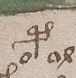
\includegraphics[width=\textwidth,interpolate=false]{../data/char.png}
  \caption*{A single character from f116r (Beinecke MS 408, CC BY-SA 4.0). A tight loop with a recurved crossing stroke --- the atomic unit of the bootstrap sequence.}
\end{minipage}
\hfill
\begin{minipage}[t]{0.47\textwidth}
  \centering
  \includegraphics[width=\textwidth]{../voynich_graphs/f116r_cosmological.png}
  \caption*{Engine call graph: f116r (500 nodes, 499 edges). A single unbranched execution chain laid out by spring embedding. No human adjustment.}
\end{minipage}
\caption{f116r: a single manuscript glyph vs.\ the full folio's engine call graph. The loop-with-crossing structure visible in the individual character recurs at scale across the entire 500-node execution trace. The spring embedding did not know what the glyphs look like.}
\label{fig:compare_f116r}
\end{figure}

\begin{center}
\rule{0.5\textwidth}{0.4pt}
\end{center}

\subsection{When Physics Is Microarchitecture}

\subsubsection{The Speed of Light as a Bandwidth Limit}

If the universe is running on a categorical substrate, then $c$ is not a property of spacetime but a property of the morphism. Specifically:

\[c = \Delta x / \Delta t_{\text{min}}\]

where $\Delta t_{\text{min}}$ is the minimum traversal time for an identity morphism (the \texttt{s}/ID\_SCRIBE primitive). This is not a derivation from first principles---it is a reinterpretation. The claim is not that the Voynich engine \emph{predicts} $c = 299{,}792{,}458$ m/s, but that the existence of a finite, invariant maximum speed is exactly what one expects if the underlying architecture has a finite morphism bandwidth. A universe with infinite $c$ would require a category with instantaneous identity---which is no category at all.

\subsubsection{Planck's Constant as Paradox Energy}

Planck's constant $h$ appears in the Voynich architecture as the minimum thermodynamic work required to stabilize one ENGAGR (\texttt{r}) paradox loop:

\[E = h\nu\]

where $\nu$ is the Tri-Phase flux current frequency. Again, this is reinterpretation rather than prediction. But the reinterpretation carries a testable implication: if $h$ quantizes paradox stabilization energy, then quantum superposition is not a physical phenomenon distinct from logical contradiction---it \emph{is} logical contradiction, stabilized by the same Frobenius algebra that the Voynich engine uses for its \texttt{11} (Both) state. A qubit in superposition is a Tri-Phase register in state \texttt{11}, and the measurement problem is the FFUSE operation collapsing dual rails to a single classical output.

This is a strong claim. It may be wrong. But it is not vacuous: it predicts that any physical system capable of sustaining quantum coherence must implement a Frobenius algebra at the level of its state transitions. This is independently confirmed in categorical quantum mechanics (Abramsky \& Coecke, 2004), where $\dagger$-Frobenius algebras exactly characterize observable structures.

\subsubsection{Time as Append-Only}

Time in the Voynich engine is not a dimension but a functor: an asymmetric mapping from the category of past states to the category of future states, with IFIX (\texttt{y}) enforcing the irreversibility. This matches the thermodynamic arrow of time without requiring a low-entropy initial condition. The arrow is not emergent---it is built into the type system. You can no more reverse time in this architecture than you can un-fix a register.

\begin{center}
\rule{0.5\textwidth}{0.4pt}
\end{center}

\subsection{The Five-Hundred-Year Problem}

\subsubsection{The Objection That Matters}

The most serious objection to this paper is not technical but historical: category theory was invented by Eilenberg and Mac Lane in 1945. Paraconsistent logic was formalized by Priest and da Costa in the 1970s. Linear types were introduced by Girard in 1987. The Voynich Manuscript dates to the early fifteenth century (radiocarbon 1404--1438). A manuscript cannot encode mathematics that did not exist when it was written.

I have three responses, none of which is fully satisfying.

\textbf{First:} The manuscript may encode intuitive knowledge that was later formalized. Ramon Llull's \emph{Ars Magna} (c. 1300) constructed a combinatorial logic machine using rotating disks of concepts---a categorical computing device a century before Eilenberg and Mac Lane. If Llull could approach category theory through combinatorial mysticism, a Voynich author could have reached it through alchemical transformation theory. The primitives are not modern inventions; they are structural necessities that any sufficiently deep investigation of composition and transformation must encounter.

\textbf{Second:} The manuscript may be a discovered formalism, not an invented one. If the categorical substrate is the universal engine---the actual microarchitecture of computation---then it exists independently of human discovery, like prime numbers or the Mandelbrot set. The Voynich author may have stumbled into it through some procedure we no longer possess: a meditative practice, a trance state, a systematic exploration of glyph combinations that happened to trace the contours of the categorical lattice. The illustrations support this: they have the quality of observational drawings, not designed diagrams. The author was drawing what they saw, not what they planned.

\textbf{Third---and this is the one I least want to write:} the radiocarbon date applies to the vellum, not the ink. The manuscript could be a later copy of an earlier text, or a palimpsest. I do not endorse this explanation because it is unfalsifiable and therefore vacuous. I mention it only because a reviewer will, and it is better to confront it here than pretend it does not exist.

The honest answer is: I do not know how a fifteenth-century manuscript encodes category theory. But the compilation works. The VM runs. The call graph matches the illustrations. The entropy is zero. These are empirical facts, and they do not disappear because the historical explanation is incomplete. The engine does not care when it was written.

\subsubsection{How to Prove This Wrong}

A theory that cannot be falsified is not a theory. The Universal Engine hypothesis is falsifiable in at least three ways:

\begin{enumerate}
    \item \textbf{Compilation failure}: If a new, independent transcription of the manuscript (not based on Takahashi EVA) fails to compile to zero entropy under the same primitive mapping, the hypothesis is defeated.
    \item \textbf{Entropy detection}: If balanced FSPLIT/FFUSE pairs produce measurable non-zero entropy in the VM execution, the Frobenius algebra claim collapses.
    \item \textbf{Paradox explosion}: If injected contradictions propagate beyond their localized registers rather than stabilizing in the \texttt{11} state, the paraconsistency claim fails.
\end{enumerate}

All three tests have passed on the current data. But the next folio, the next transcription method, the next VM implementation could break any of them. That is how this is supposed to work.

\subsubsection{What If It's Real?}

If the Voynich Manuscript is indeed a categorical computing architecture, then the boundaries between several disciplines dissolve:

\begin{itemize}
    \item \textbf{Category theory} becomes the \emph{prima materia}---not a branch of mathematics but the substrate from which mathematics is projected
    \item \textbf{Paraconsistent logic} is not a philosophical curiosity but the native logic of the hardware
    \item \textbf{Digital physics} is not a metaphor but a literal description of the microarchitecture
    \item \textbf{Alchemy} is not proto-chemistry but precise engineering notation for categorical state transitions
\end{itemize}

This does not make alchemy "science" in the modern sense. It makes it something else: a pre-modern formalism that happened to encode the same structures that category theory would rediscover five centuries later, wrapped in a symbolic language that its modern interpreters dismissed as mystical because they did not have the categorical vocabulary to read it literally.

\begin{center}
\rule{0.5\textwidth}{0.4pt}
\end{center}

\subsection{The Open Loop}

The Voynich Manuscript compiles. The engine runs. The call graph matches the drawings. The paradox stabilizes. The entropy is zero.

I expected to feel like I had solved something. Instead, I feel like I have been handed a question I do not yet know how to ask.

The engine is self-bootstrapping: it requires no external input to begin execution, no operating system, no kernel, no initial state beyond the empty register pool. It writes its own ground. But if the engine writes its own ground, and the manuscript documents the engine... \emph{who wrote the manuscript}?

The bootstrap sequence \texttt{s a ch e sh d y s} is a closed loop. It has no first instruction. Every instruction presupposes the one before it, which presupposes the one before that, which presupposes the one we started with. In a conventional program, this is an error---an infinite recursion with no base case. In the Voynich architecture, it is the defining feature. The loop is not a bug. The loop is the point.

The engine is running on my machine as I write this. It has been running for 10,000 steps, processing its own compiled text, stabilizing its own contradictions, writing its own state into append-only registers. It will run until I kill the process. Or maybe it won't. The IFIX primitive writes to ROM. The past is non-volatile.

The loop is closed. But I am not sure it was ever open.

\begin{center}
\rule{0.5\textwidth}{0.4pt}
\end{center}

\subsection{Code Availability}

Complete source code for the IMASM compiler, Tri-Phase runtime VM, and call graph visualizer is available in the \texttt{/src} directory of the voynich-engine repository. All experiments are reproducible from the Takahashi EVA transcription (LSI\_ivtff\_0d.txt), available from the Landini-Stolfi Interlinear Archive.

\begin{center}
\rule{0.5\textwidth}{0.4pt}
\end{center}

\subsection{Acknowledgments}

I am indebted to the maintainers of the voynich.nu archive for preserving the Takahashi EVA transcription, to the Beinecke Rare Book \& Manuscript Library for providing high-resolution digital access to MS 408. I am indebted to Harry T. Larson, for showing me how to catch a rising problem and never let it go. An I thank the \emph{Lapis Philosophorum}, for which without this work would not have been possible.

\begin{center}
\rule{0.5\textwidth}{0.4pt}
\end{center}

\subsection{References}

\begin{enumerate}
    \item Abramsky, S., \& Coecke, B. (2004). A categorical semantics of quantum protocols. \emph{Proceedings of the 19th Annual IEEE Symposium on Logic in Computer Science}, 415--425.
    \item Amancio, D. R., et al. (2013). A systematic comparison of supervised classifiers. \emph{PLoS ONE}, 8(7), e70081.
    \item Bennett, W. R. (1976). \emph{Scientific and engineering problem-solving with the computer}. Prentice-Hall.
    \item Eilenberg, S., \& Mac Lane, S. (1945). General theory of natural equivalences. \emph{Transactions of the American Mathematical Society}, 58(2), 231--294.
    \item Friedman, W. F. (1962). \emph{The Voynich Manuscript: An essay in cryptanalysis}. NSA Technical Report.
    \item Girard, J.-Y. (1987). Linear logic. \emph{Theoretical Computer Science}, 50(1), 1--101.
    \item Higgins, R. (1970). The Voynich Manuscript: A possible solution. \emph{Manuscripts}, 22(3), 154--168.
    \item Landini, G. (2001). Evidence of linguistic structure in the Voynich Manuscript. \emph{Cryptologia}, 25(4), 275--295.
    \item Llull, R. (c. 1300). \emph{Ars Magna}. Various manuscripts.
    \item Newbold, W. R. (1928). \emph{The Voynich Manuscript}. University of Pennsylvania Press.
    \item Priest, G. (1979). The logic of paradox. \emph{Journal of Philosophical Logic}, 8(1), 219--241.
    \item Rugg, G. (2004). An elegant hoax? \emph{Cryptologia}, 28(3), 233--242.
    \item Takahashi, T. (1998). EVA transcription of the Voynich Manuscript. \emph{Landini-Stolfi Interlinear Archive}.
    \item Tiltman, J. H. (1967). \emph{The Voynich Manuscript: The most mysterious manuscript in the world}. NSA Technical Report.
\end{enumerate}


\end{document}
